%% 062Analyse.tex
%% $Id: 062Analyse.tex 4 2005-10-10 20:51:21Z bless $
%%

%% ==============================
\subsection{Angaben der Probanden}
%% ==============================

\begin{figure}[htbp] 
	\centering
	\begin{minipage}[t]{0.4\textwidth}
		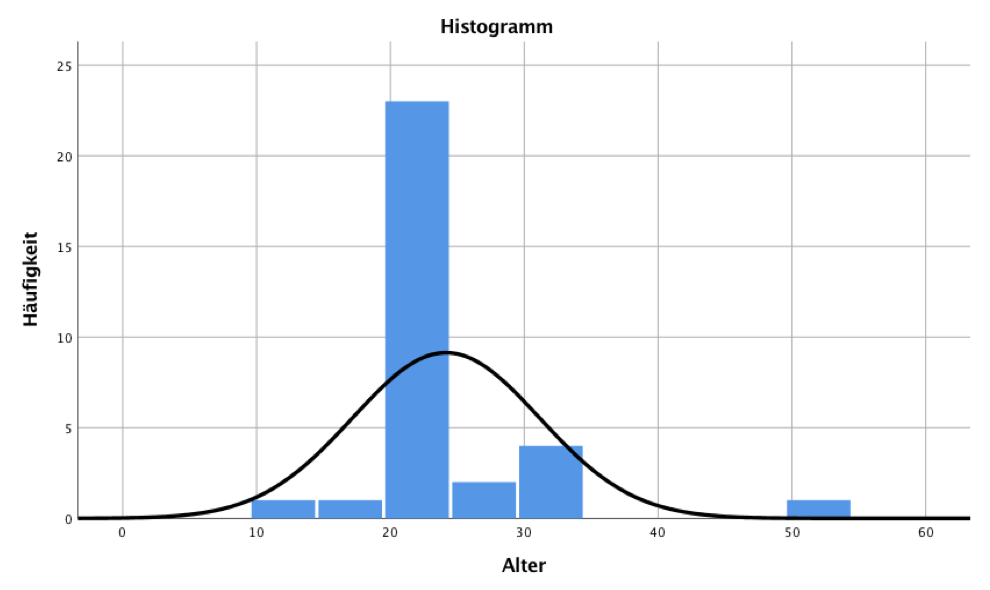
\includegraphics[width=\textwidth]{pics/analyse/person/alter.png}
	\end{minipage}
	\begin{minipage}[t]{0.4\textwidth}
		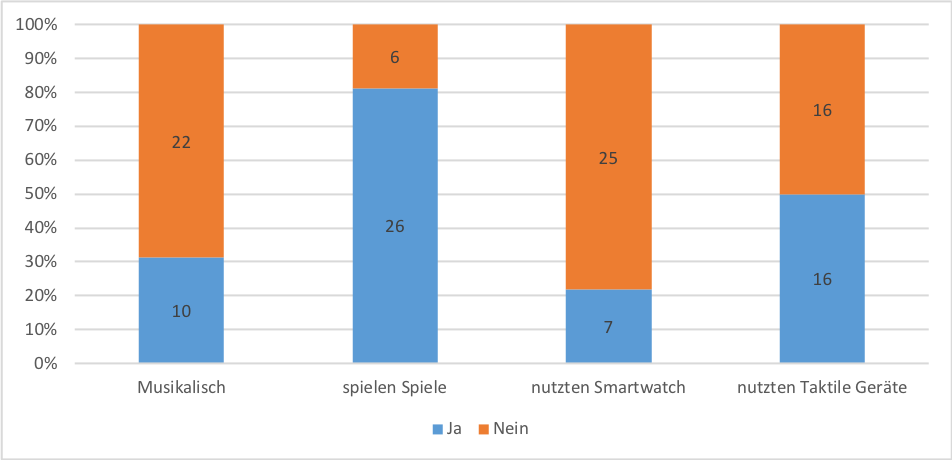
\includegraphics[width=\textwidth]{pics/analyse/person/questions.png}
	\end{minipage}
	\caption{Alter aller Probanden (links) und Auswertung der Fragen (rechts)}
	\label{fig:AngabenZurPerson}
\end{figure}

Nach der Befragung der Probanden hat sich ergeben, dass 31\% musikalisch sind, 81\% gelegentlich Computerspiele spielen. 21\% haben schon mal eine Smartwatch benutzt und genau die h{\"a}lfte haben schon mal taktile Ger{\"a}te benutzt.

%% ==============================
\subsection{Initialisierung der Grenzen}
%% ==============================
\label{ch:Evolution{\"a}rer Algorithmus:sec:Studiendesign}

\begin{figure}[htbp] 
            \centering
   	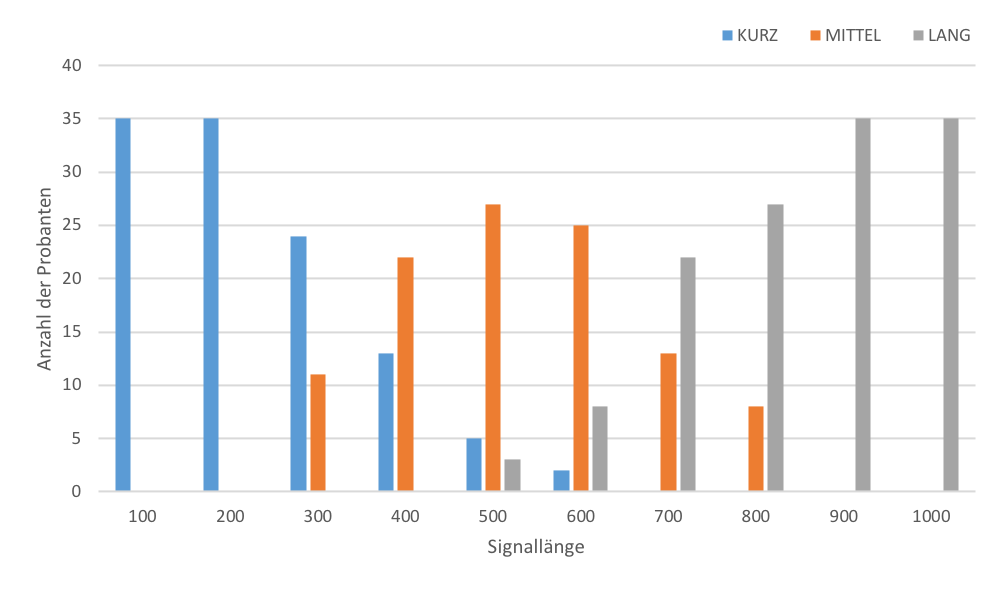
\includegraphics[width=\textwidth]{pics/analyse/Initialisierung.png}
	\caption{}
	\label{fig:Initialisierung}
\end{figure}

F{\"u}r die Bestimmung der Grenzen von Kurz, Mittel und Lang hat der Benutzer 10 Signale zu der jeweiligen Kategorie einordnen sollen. 
Da man bei 16\% der Probanden bei diesem Schritt keine eindeutigen Grenzen bestimmen konnte, musste der Schritt ein weiteres mal wiederholt werden. 

Obwohl die 10 normalverteilten Signale in zuf{\"a}lliger Reihenfolge abgespielt wurden, wurde bei 84\% aller Probanden die zehn Signale so bewertet, dass zuerst alle Kurz, gefolgt von nur Mittel und anschlie{\ss}end nur Lang bewertet wurden. Die restlichen Probanden haben an den Grenzen nur ein Signal von Kurz und Mittel oder Mittel und Lang vertauscht gehabt.

%Au{\ss}erdem ist bei 84\% aller Probanden die Zuordnung der Kategorie zu den Signalen so bewertet worden, dass zuerst eine Anzahl von Signalen als Kurz, gefolgt von einer weiteren Anzahl als Mittel und schlie{\ss}lich der Rest als Lang erkannt worden ist.
%dass zuerst alle Signale als Kurz, gefolgt von nur Signale als Mittel und schlie{\ss}lich nur Signale vom Langen . 

%Die restlichen 16\% der Probanden haben an den Grenzen der Signaltypen nur ein Signal vom Kurz und Mittel oder Mittel und Lang vertauscht gehabt.

In der Auswertung\ref{Initialisierung} haben sich drei Normalverteilungen gebildet. Daraus kann man entnehmen, dass Werte 100ms und  200 ms eindeutig als Kurz, sowie auch Werte 900ms und 1000ms als Lang erkannt worden sind. Einen eindeutigen Hochpunkt f{\"u}r Mittel hat man bei dem Wert von 500ms, dennoch gab es einige Probanden f{\"u}r die dieser Wert noch als Kurz oder Lang empfunden wurde. 

Aus dem Diagramm kann man sehr sch{\"o}n erkennen, dass man eine Personalisierung von Vibrationen ben{\"o}tigen k{\"o}nnte, da au{\ss}er den R{\"a}ndern keine Eindeutige Zuweisung von Kurz, Mittel oder Lang passieren konnte. Man kann zwar im Vorfeld Werte f{\"u}r Signale definieren, wie es derzeitig einige Firmen machen, diese Werte k{\"o}nnten jedoch von Personen unterschiedlich wahrgenommen werden.
%Aus dem Diagramm kann man sehr sch{\"o}n erkennen, dass man Werte zwar im Vorfeld selbst definieren kann, diese Werte k{\"o}nnten unter verschiedenen Probanden jedoch anders wahrgenommen werden und es wei{\ss}t darauf hin, dass man sehr wohl eine Personalisierung von Vibrationen ben{\"o}tigen k{\"o}nnte. 

%% ==============================
\subsection{Auswertung der Iterationen des Algorithmus}
%% ==============================


\paragraph{Verlauf der Grenzen}

\begin{figure}[htbp] 
	   \centering
   	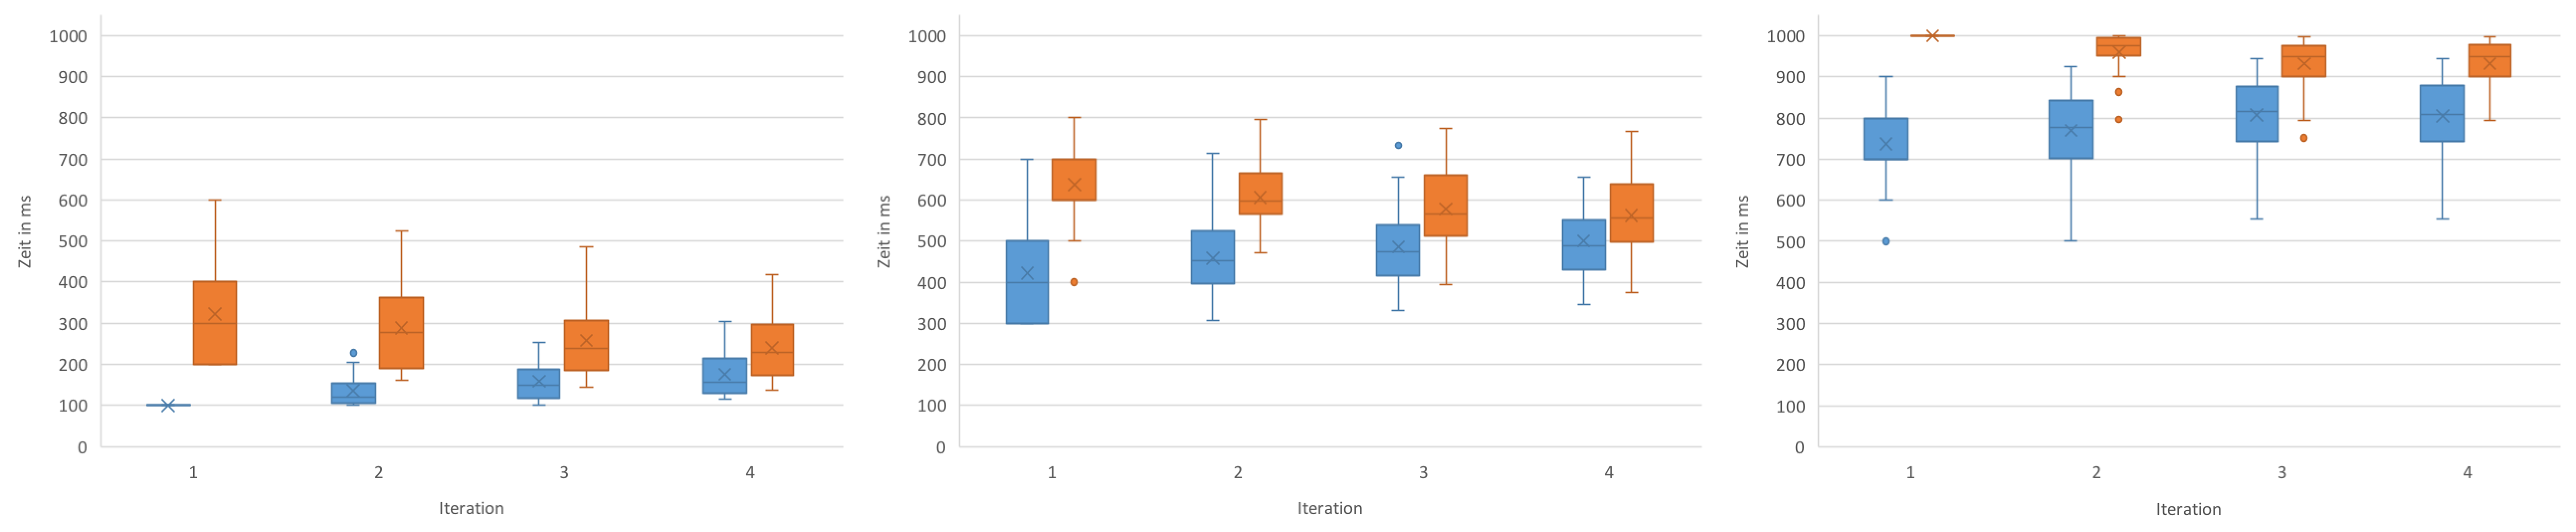
\includegraphics[width=\textwidth]{pics/analyse/algo/MinMax/MinMaxFinal.png}
	\caption{Darstellung des Minimum (in blau) und Maximum (in rot) im Verlauf der 4 Iterationen des Algorithmus. Das erste Bild zeit Kurz, gefolgt von Mittel und Lang.}
	\label{fig:MinMaxSignale}
\end{figure}

Der Algorithmus wurde insgesamt vier mal ausgef{\"u}hrt, anschlie{\ss}end wurde aus der letzten Population der personalisierte Wert gemittelt. 

\paragraph{Kurz}
Eine der gr{\"o}{\ss}ten Ver{\"a}nderungen im Diagramm \autoref{MinMaxSignale} gibt es bei \textbf{Kurz}; die oberste Grenze vom Maximum ist nach vier Iterationen von 600ms auf 415ms gesunken. Die obere Grenze des Minimum ist von 100ms auf 300ms gestiegen. 
Der Bereich verkleinert sich insgesamt vom Intervall von 100 bis 600ms auf 140 bis 420 ms. 
Der Median von den Maximum und Minimum konvergieren in die gleiche Richtung. Nach vier Iterationen ist der Median vom Minimum um 80ms nach oben und der Median von dem Maximum auch um 80ms nach unten gewandert. 
Das Minimum und Maximum {\"u}berschneidet sich in der 2. Iteration nur minimal. In der 4. Iteration sich Minimum und Maximum um 150ms {\"u}berschneiden. Das 50\% Quartil vergr{\"o}{\ss}ert sich auf ein Intervall bis zu 100ms, wobei das 50\% Quartil von einem 20ms Intervall auf ein 120ms Intervall verdichtet. 


\paragraph{Mittel}
In der ersten Iteration besitzt man schon {\"u}berschneidungen des Minimum und Maximum. Von der ersten zur zweiter Iteration verschieben sich die Grenzen des Minimum um ca. 10 ms nach oben, diese werden im Verlauf zur dritten und vierten Iteration kleiner.  Die Grenzen des Maximums hingegen werden gr{\"o}{\ss}er und verschieben sich anschlie{\ss}end minimal nach unten. Das 50\% Quartil ver{\"a}ndert sich beim Minimum von einem 200ms Intervall auf ein 120ms Intervall und verschiebt sich anschlie{\ss}end im Verlauf der folgenden Iterationen nur nach oben. 

\paragraph{Lang}
Die meisten Ausrei{\ss}er sind in bei Lang vertreten, hier hat man in der zweiten Iteration schon ein Maximum von 1000ms auf unter 800ms und 880ms erhalten, das ist eine {\"a}nderung eines Maximums um 200ms nach nur einer Iteration bei einem Probanden.
Die 50\% Quartile des Maximums werden Minimal gr{\"o}{\ss}er und wachten nach unten.
Bei den 50\% Quartile des Minimums werden die kurzzeitig gr{\"o}{\ss}er {\"a}ndern sich aber wieder auf mit dem Ausrei{\ss}er der ersten Iteration auf das gleiche Intervall und verschieben sich pro Iteration leicht nach oben.


\\

Unter den Signaltypen selbst {\"u}berschneiden sich die Iterationen die Grenzen selbst zwischen den Iterationen selbst. Diese {\"u}berschneidungen verringern sich nach den 4 Iterationen.

Das Minimum steigt stetig und das Maximum verringert sich. Denn genau diesen Effekt wollte man auch erzielen, dass der Benutzer zu seinen personalisierten Wert konvergiert.
Bei Kurz und Mittel {\"u}berschneiden sich die 50\% Quartile. Bei Lang {\"u}berschneiden diese in keiner Iteration.

Schlussfolgernd kann man sagen, dass die man anhand der 50\% Quartile vom Maximum und Minimum aller Probanden einen Kurzes Signal in dem Bereich von 130ms bis 300ms, ein Mittleres Signal zwischen 430ms und 640ms und ein Langes Signal zwischen 740ms und 980ms die gebildet haben. 


\paragraph{Grenzen nach dem Algorithmus}

\begin{figure}[htbp] 
            \centering
   	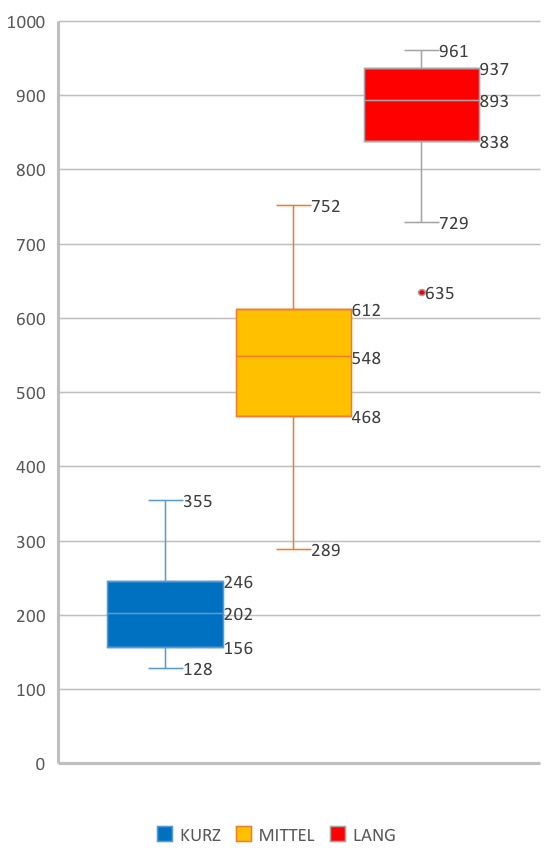
\includegraphics[width=\textwidth]{pics/analyse/algo/MinMax/GrenzenNachAlgo.png}
	\caption{Nach der Vierten Iteration gemittelte personalisierte Werte in ms}
	\label{fig:GrenzenNachAlgo}
\end{figure}

In dem Diagramm \autoref{GrenzenNachAlgo} sind alle gemittelten personalisierten Werte nach der vierten Iteration abgebildet. 
Daraus l{\"a}sst sich ableiten, dass zwischen den Kategorien von Kurz, Mittel und Lang sich die Grenzen {\"u}berschneiden.
F{\"u}r die Einzelnen Kategorien hat sich der Median f{\"u}r Kurz bei 202ms, f{\"u}r Mittel bei 548ms und Lang bei 893ms festgelegt.
Die oberen 25\% bei Lang und die unteren 25\% von Kurz weisen nur eine minimale Abweichung auf. 
Im Gegensatz dazu gibt es eine Abweichung von genau 109ms bei den oberen 25\% von Kurz und den unteren 25\% von Lang.
Die Grenzen {\"u}berschneiden sich von Kurz und Mittel zwischen 289ms bis 355ms und von Mittel und Lang zwischen 729ms und 752ms.
Es gibt einen Ausrei{\ss}er bei Lang mit einem Wert von 635ms, dabei handelt es sich nicht um keinen Fehler, sondern einen Probanden der genau dies f{\"u}r sich als Personalisierten Wert bestimmt hat.
Im Vergleich der inneren 50\% von den jeweiligen Kategorien wei{\ss}t Kurz einen Intervall von 90 ms und Lang einen Intervall von 99ms auf, wobei Mittel diesen Wert von 144 ms am gr{\"o}{\ss}ten Bereich ist und um nahezu 50ms gr{\"o}{\ss}er als Kurz und Lang ist. 


\paragraph{Stimmung im Verlauf des Algorithmus}

\begin{figure}[htbp] 
            \centering
   	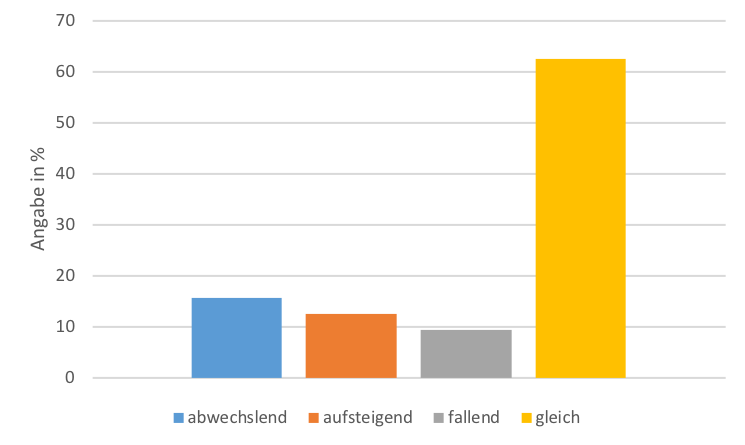
\includegraphics[width=\textwidth]{pics/analyse/person/Stimmung.png}
	\caption{Bewertung der Stimmung}
	\label{fig:Stimmung}
\end{figure}

Nach jeder Iteration wurden die Benutzer gefragt wie Ihre Stimmung \autoref{Stimmung} aktuell sei. Dabei hat es bei 62\% aller Probanden keine {\"a}nderung der Stimmung  gegeben. Diese Probanden hatten Ihre Stimmung mit \textbf{Gut} oder \textbf{Sehr gut} bewertet gehabt. Im Gegensatz dazu hat sich die Stimmung bei 16\% der Probanden entweder zwischen \textbf{Gut} und \textbf{Sehr gut} oder \textbf{Gut} und \textbf{OK} abgewechselt. Des Weiteren gab es bei 13\% der Probanden eine aufsteigende Stimmung und bei den restlichen 9\% ist die Stimmung pro Iteration gefallen.

Somit kann man feststellen, dass die Anzahl von vier Iterationen keinen wirklichen Einfluss auf die Stimmung des Benutzers ausgewirkt hat.

% die ben{\"o}tigt wurde um den Algorithmus auszuf{\"u}hren, sich nicht auf die Stimmung Stimmung sich nicht  ausgewirkt hat. 

\paragraph{Replays eines Signals}

\begin{figure}[htbp] 
            \centering
   	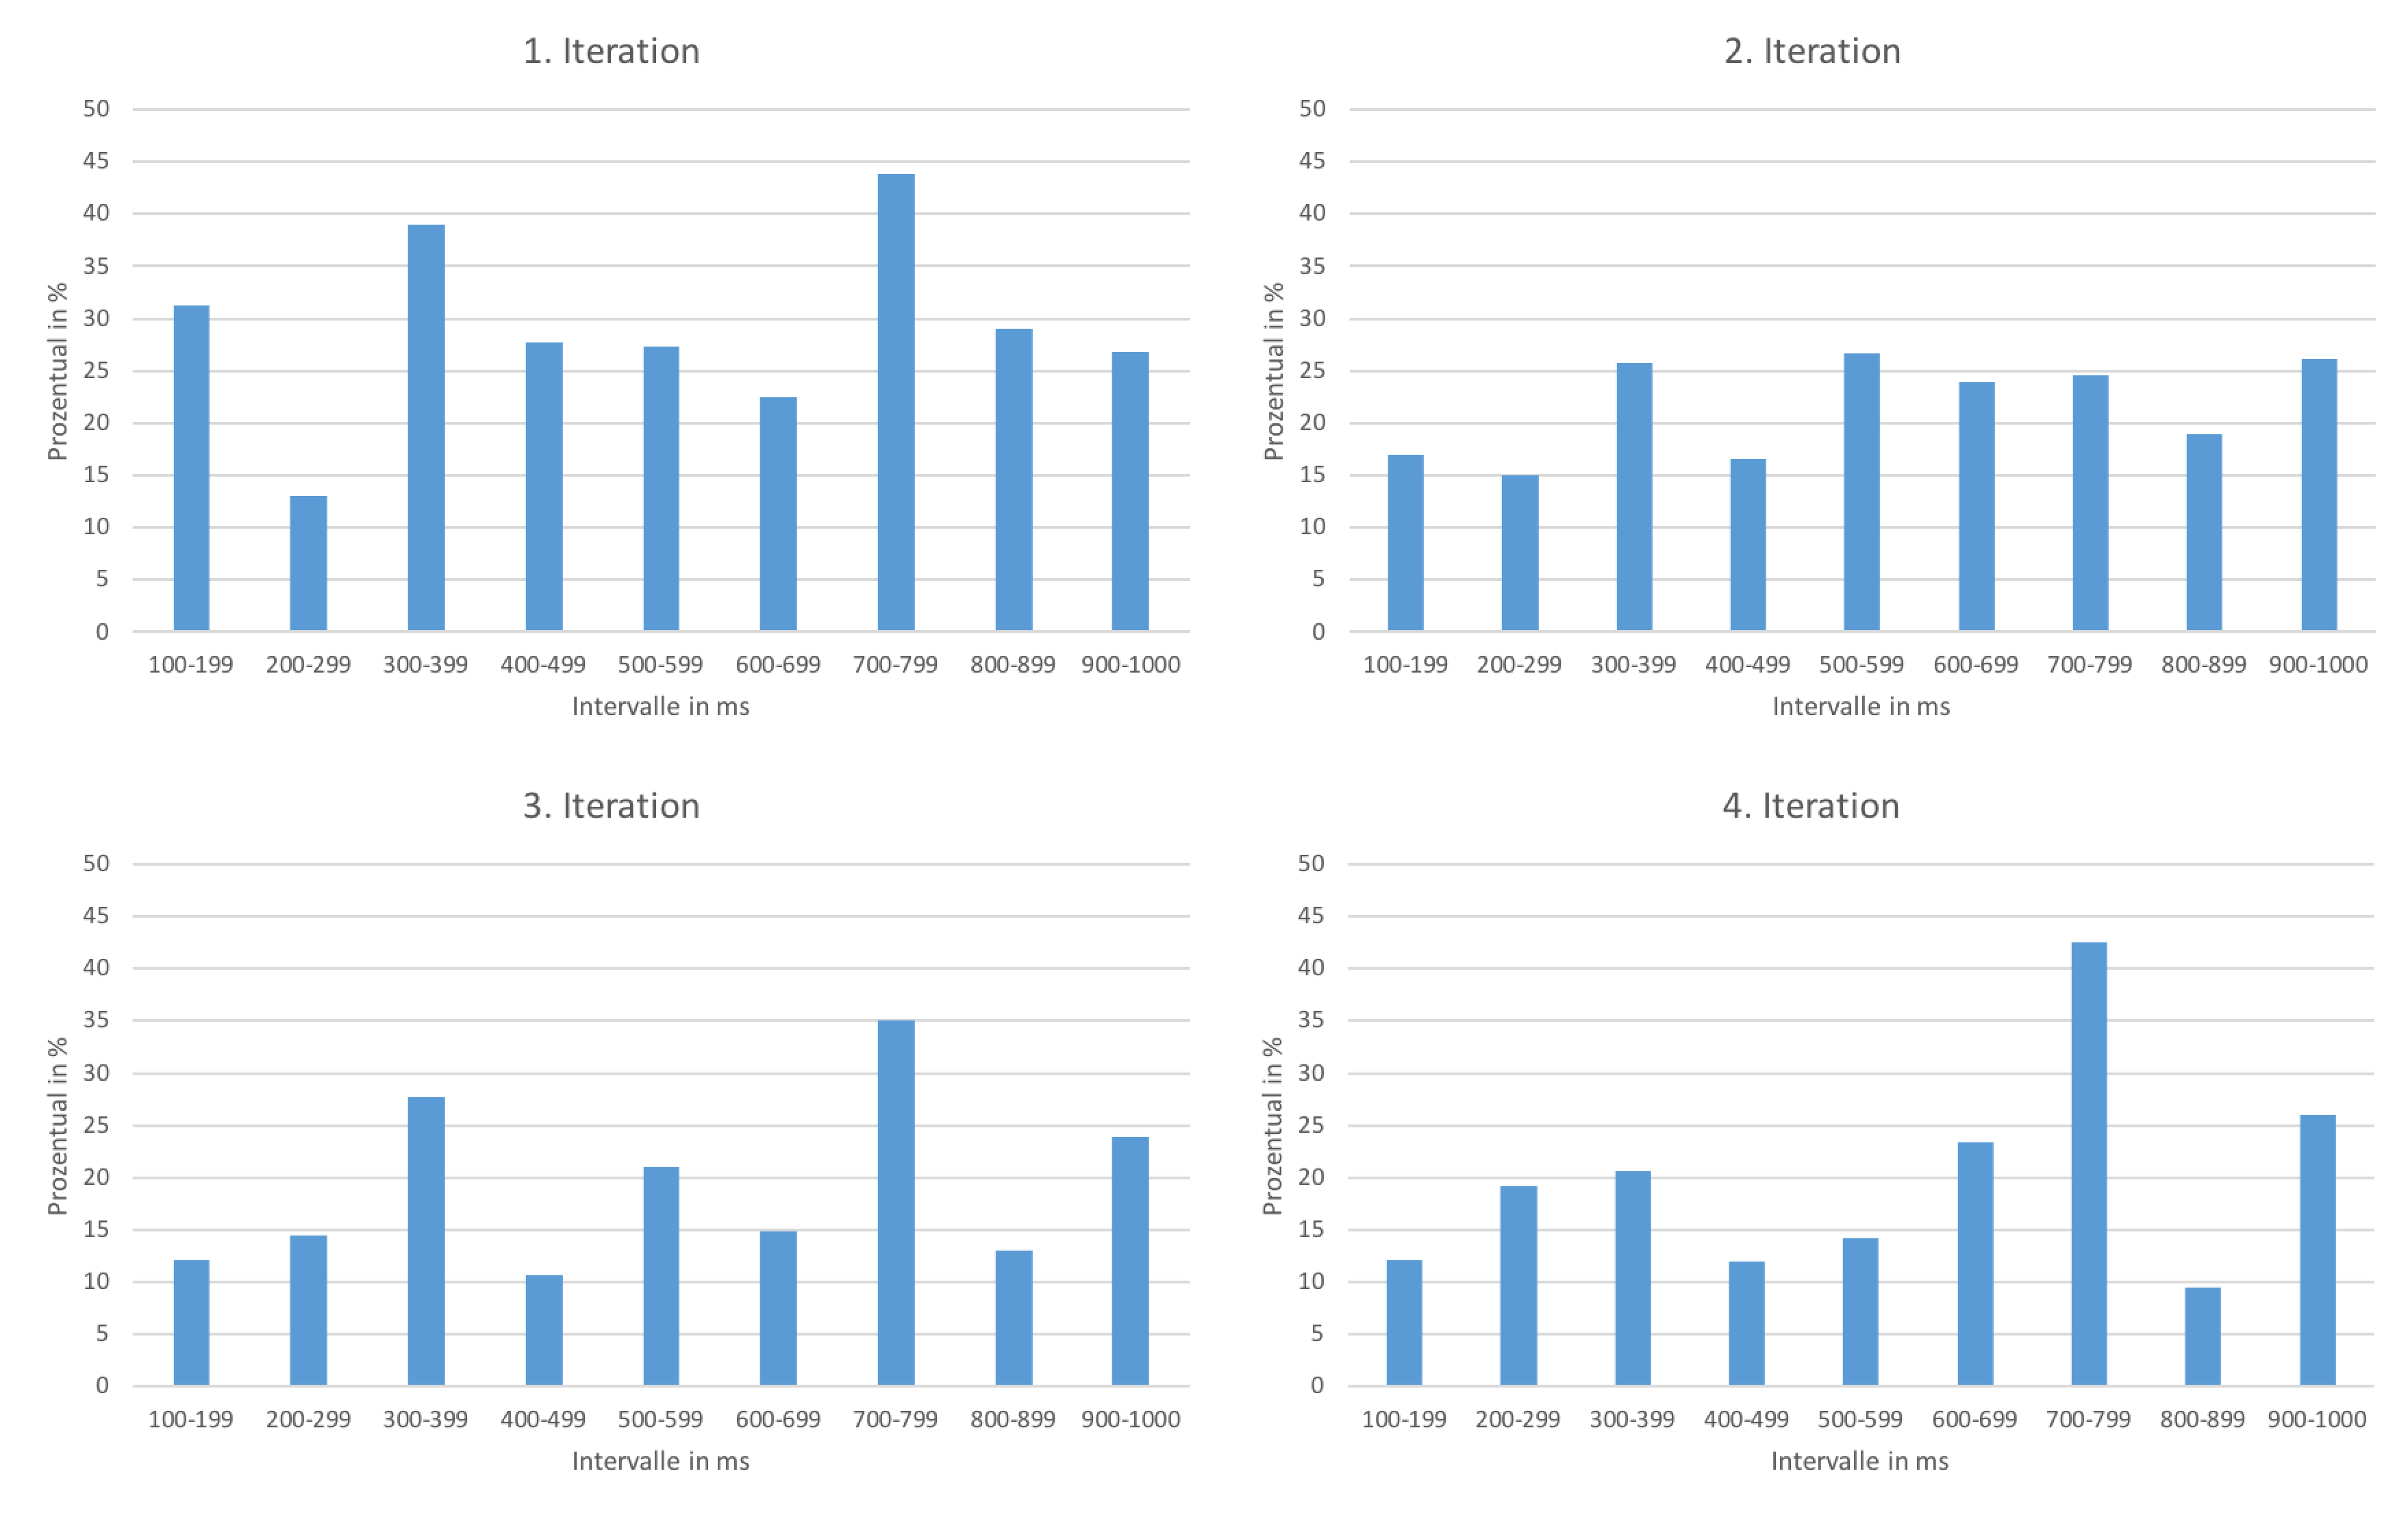
\includegraphics[width=\textwidth]{pics/analyse/algo/Replay/ReplayFinal2.png}
	\caption{Anzahl der Replays innerhalb von Zeitintervallen {\"u}ber dem Verlauf des Algorithmus}
	\label{fig:ReplayFinal}
\end{figure}

Man hat dem Probanden die M{\"o}glichkeit geboten, ein Signal wiederholen zu d{\"u}rfen. Im Verlauf des Algorithmus wollte man herausfinden wie oft unter allen Probanden auf Replay f{\"u}r ein bestimmten Intervall Replay gedr{\"u}ckt wurde \autoref{ReplayFinal}. Die Anzahl der wie oft auf Replay gedr{\"u}ckt wurde 

In der ersten Iteration haben 44\% der Probanden in dem Intervall von 700-799ms die gr{\"o}{\ss}ten Schwierigkeiten gehabt ein Signal zuzuordnen und sich das Signal erneut abgespielt. Der Bereich, der am wenigsten wiederholt abgespielt werden musste war 200-299ms. Die Restlichen Intervalle der ersten Iteration wurden mit einem Mittelwert von 32\% erneut abgespielt.

In der zweiten Iteration hat sich die Anzahl der Replays um einiges geringer hier war der Mittelwert insgesamt bei 22\% mit einem Minimum bei 200-299ms von 15\% und einem Maximum bei 500-599ms mit 27\%.  Die dritte Iteration hat eine Verbesserung bei allen nahezu allen Werten gehabt, bis auf das Intervall von 700-799ms was auf 35\% angestiegen ist; insgesamt ist der Mittelwert in dieser Iteration bei 19\%. 

Selbst in der letzten Iteration hat sich ein globales Minimum bei 800-899ms von 9,5\% gebildet. Der globale Maximum von 700-799 in der ersten Iteration mit 43\% ist auch in der vierten Iteration, trotz Verbesserungen zwischen durch, auch das Maximum mit 42,5\%. 

Man kann daraus erkennen, dass die Probanden genau an dem Bereich von Kurz zu Mittel, was sich in der 4. Iteration bei 200-399ms bewegt, und Mittel zu Lang, dass zwischen 600-799ms liegt, am meisten den Replay Knopf gedr{\"u}ckt haben. Ein viertel aller Probanden haben bei 900-1000ms in jeder Iteration das Signal erneut abgespielt. Jedoch kann man in der vierten Iteration sehr gut erkennen, dass die Signale mit den  Werten 100-199ms, 400-599ms und 800-899ms am geringsten erneut abgespielt werden mussten.
Im Schnitt wurde, falls man ein Signal erneut abgespielt haben wollte, 1,7mal der Replay Button gedr{\"u}ckt, bei einem Minimum von einmal und einem Maximum von 9 mal, im Verlauf des Algorithmus. 




